\pdfminorversion=4
\documentclass[aspectratio=169]{beamer}

\mode<presentation>
{
  \usetheme{default}
  \usecolortheme{default}
  \usefonttheme{default}
  \setbeamertemplate{navigation symbols}{}
  \setbeamertemplate{caption}[numbered]
  \setbeamertemplate{footline}[frame number]  % or "page number"
  \setbeamercolor{frametitle}{fg=white}
  \setbeamercolor{footline}{fg=black}
} 

\usepackage[english]{babel}
\usepackage[utf8x]{inputenc}
\usepackage{tikz}
\usepackage{courier}
\usepackage{array}
\usepackage{bold-extra}
\usepackage{minted}
\usepackage[thicklines]{cancel}
\usepackage{fancyvrb}

\xdefinecolor{dianablue}{rgb}{0.18,0.24,0.31}
\xdefinecolor{darkblue}{rgb}{0.1,0.1,0.7}
\xdefinecolor{darkgreen}{rgb}{0,0.5,0}
\xdefinecolor{darkgrey}{rgb}{0.35,0.35,0.35}
\xdefinecolor{darkorange}{rgb}{0.8,0.5,0}
\xdefinecolor{darkred}{rgb}{0.7,0,0}
\definecolor{darkgreen}{rgb}{0,0.6,0}
\definecolor{mauve}{rgb}{0.58,0,0.82}
\definecolor{titlecolor}{rgb}{0.25,0.34,0.74}

\title[2020-07-06-scipy2020]{\textcolor{titlecolor}{Manipulating JSON-like Data with NumPy-like Idioms}}
\author{\underline{Jim Pivarski}, Ianna Osborne, Peter Elmer}
\institute{Princeton University -- IRIS-HEP}
\date{July 7, 2020}

\usetikzlibrary{shapes.callouts}

\begin{document}

\logo{\pgfputat{\pgfxy(0.11, 7.4)}{\pgfbox[right,base]{\tikz{\filldraw[fill=dianablue, draw=none] (0 cm, 0 cm) rectangle (50 cm, 1 cm);}\mbox{\hspace{-8 cm}
\includegraphics[height=1 cm]{princeton-logo-long.png}\hspace{0.1 cm}\raisebox{0.1 cm}{
\includegraphics[height=0.8 cm]{iris-hep-logo-long.png}}\hspace{0.1 cm}}}}}

\begin{frame}
  \vspace{1.75 cm}
  \mbox{ } \hfill 
\includegraphics[width=0.4\linewidth]{logo-600px.png} \hfill \mbox{ }
  
  \vspace{-1 cm}
  \titlepage
\end{frame}

\logo{\pgfputat{\pgfxy(0.11, 7.4)}{\pgfbox[right,base]{\tikz{\filldraw[fill=dianablue, draw=none] (0 cm, 0 cm) rectangle (50 cm, 1 cm);}\mbox{\hspace{-8 cm}
\includegraphics[height=1 cm]{princeton-logo.png}\hspace{0.1 cm}\raisebox{0.1 cm}{
\includegraphics[height=0.8 cm]{iris-hep-logo.png}}\hspace{0.1 cm}}}}}

% Uncomment these lines for an automatically generated outline.
%\begin{frame}{Outline}
%  \tableofcontents
%\end{frame}

% START START START START START START START START START START START START START

%% Window capture
%% Crop top: 10
%% Crop left: 15
%% Crop right: 25
%% Crop bottom: 50

%% Audio capture
%% -10.1 dB

%% JupyterLab zoom: 200%

\begin{frame}[fragile]{What do I mean by {\it that}?}
\vspace{0.3 cm}

\small
\begin{minted}{python}
>>> import awkward1 as ak
>>> import numpy as np
\end{minted}

\begin{minted}{python}
>>> dataset = [
...     [{"x": 1,  "y": [101]},
...      {"x": 4,  "y": [102, 202]},
...      {"x": 9,  "y": [103, 203, 303]}],
...     [],
...     [{"x": 16, "y": [104, 204, 304, 404]},
...      {"x": 25, "y": [105, 205, 305, 405, 505]}]
... ]
>>> array = ak.Array(dataset)
\end{minted}

\begin{uncoverenv}<2->
\begin{minted}{python}
>>> array[2, :, "y", -1]
<Array [404, 505] type='2 * int64'>
\end{minted}
\end{uncoverenv}

\begin{uncoverenv}<3->
\begin{minted}{python}
>>> array[:, :, "y", 0] - np.sqrt(array[:, :, "x"])
<Array [[100, 100, 100], [], [100, 100]] type='3 * var * float64'>
\end{minted}
\end{uncoverenv}
\end{frame}

\begin{frame}{Table of contents}
\vspace{0.4 cm}

\large
\begin{description}\setlength{\itemsep}{0.15 cm}
\item[1:00\hspace{0.5 cm}] \textcolor{gray}{(This table of contents)}
\item[2:00\hspace{0.5 cm}] Why does this library exist? Motivation from particle physics
\item[5:00\hspace{0.5 cm}] ``Live'' demo exploring a dataset: Chicago bike paths
\item[10:00\hspace{0.5 cm}] Data types and how we generalize NumPy
\item[13:00\hspace{0.5 cm}] Using Awkward Arrays in Numba
\item[15:00\hspace{0.5 cm}] Building arbitrary structures (still in Numba)
\item[17:00\hspace{0.5 cm}] Interoperability with Pandas, Arrow, NumExpr\ldots
\item[18:00\hspace{0.5 cm}] How it works: columnar transformations
\item[20:00\hspace{0.5 cm}] Software architecture from Awkward 0.x to 1.x
\item[23:00\hspace{0.5 cm}] Development of a GPU backend
\item[25:00\hspace{0.5 cm}] Conclusions
\end{description}
\end{frame}

\begin{frame}{}
\Huge
\vspace{1 cm}
\begin{center}
\textcolor{darkblue}{Why does Awkward Array exist?}

\vspace{0.25 cm}
\textcolor{darkblue}{Motivation from particle physics}
\end{center}
\end{frame}

\begin{frame}{Example of a particle physics analysis}
\large
\begin{columns}
\column{0.48\linewidth}
\vspace{0.3 cm}
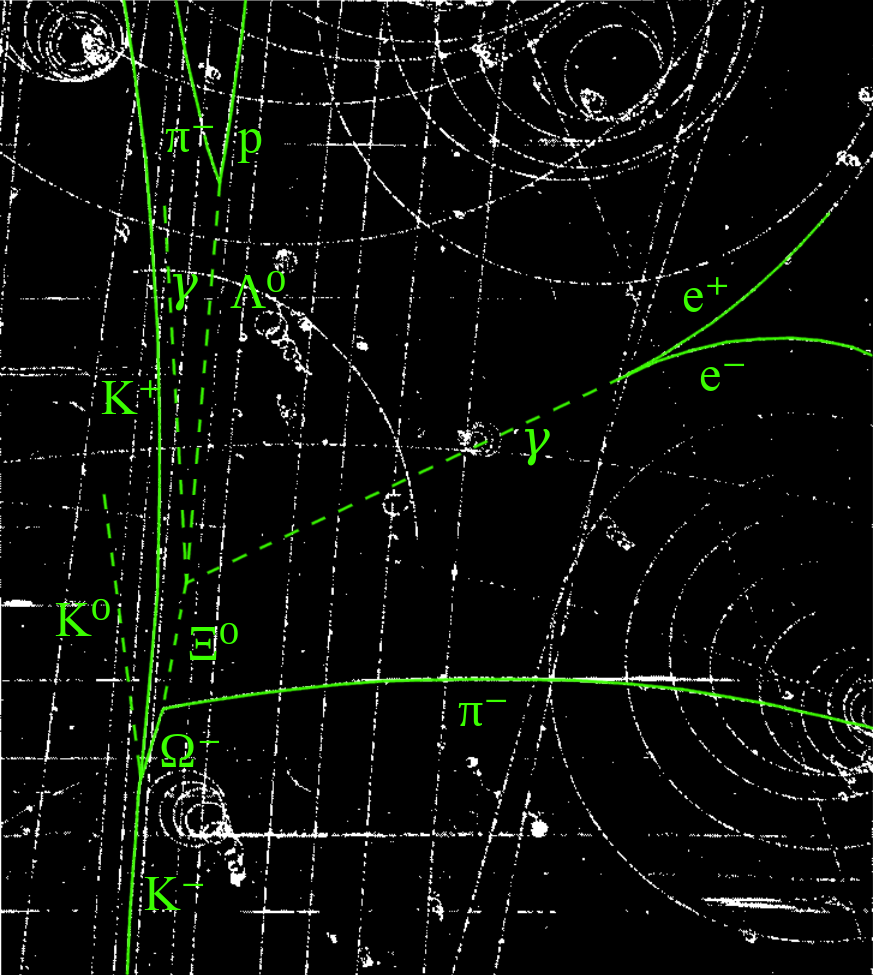
\includegraphics[width=\linewidth]{img/omega-minus-2.png}
\column{0.55\linewidth}

\begin{center}
In 1964, a group at Berkeley sifted through 100,000 photos to find this one: tracks left by decay products of an $\Omega$ baryon.

\vspace{0.25 cm}
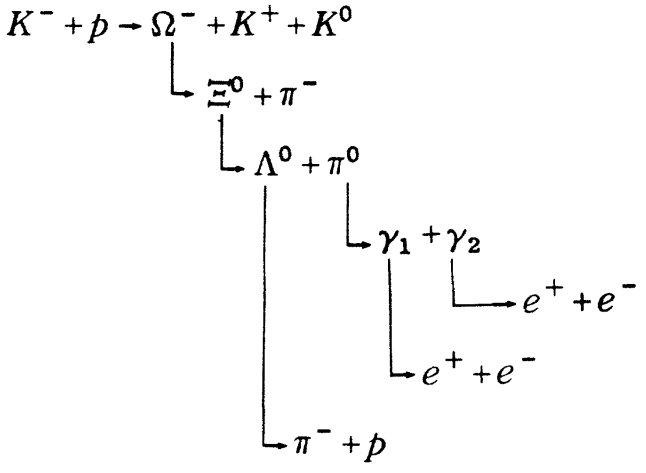
\includegraphics[width=\linewidth]{img/decay-chain.png}
\end{center}

\end{columns}
\end{frame}

\begin{frame}{Today: the same {\it kind} of thing, but bigger}
\vspace{0.15 cm}
\begin{columns}
\column{0.32\linewidth}
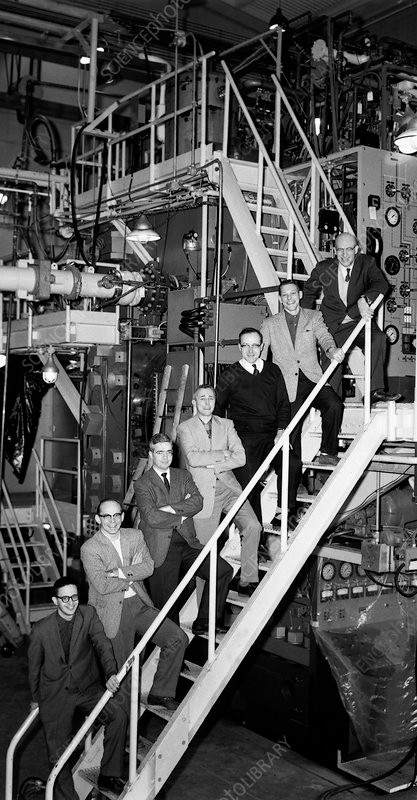
\includegraphics[width=\linewidth]{img/H4000010-Team_that_discovered_Omega_minus_particle.jpg}

\column{0.5\linewidth}
\begin{center}
\begin{columns}
\column{0.35\linewidth}
\centering
\vspace{-1 cm}

photographs

\vspace{\baselineskip}
\vspace{0.5 cm}
100,000 events

\vspace{0.5 cm}
manual/semi-automated scans

\vspace{\baselineskip}
\vspace{0.5 cm}
30 authors

\column{0.35\linewidth}
\centering
\vspace{-1 cm}

digitized signals \\

\vspace{0.5 cm}
$\sim$trillion events \\

\vspace{0.5 cm}
algorithmic searches and machine learning

\vspace{0.5 cm}
3,000 authors
\end{columns}
\end{center}

\column{0.32\linewidth}
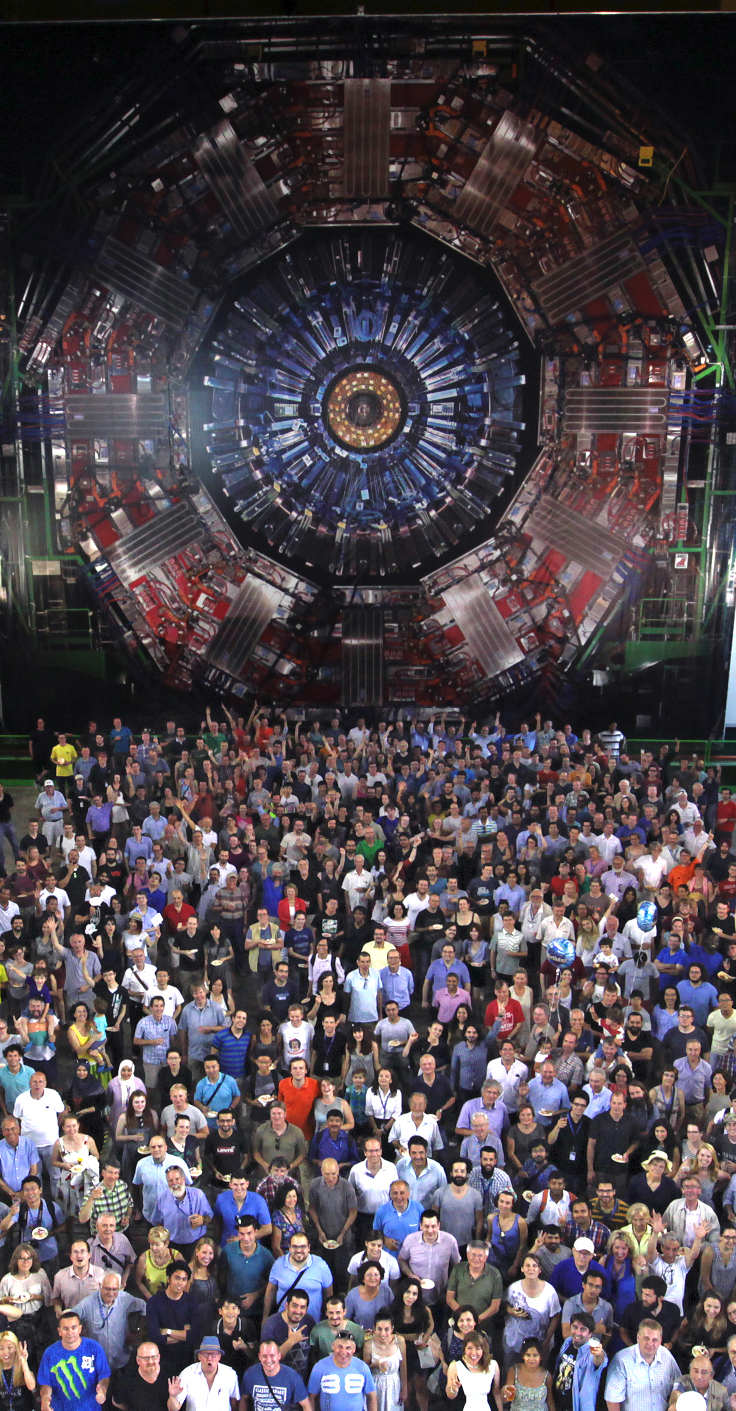
\includegraphics[width=\linewidth]{img/cms25_2.jpg}
\end{columns}
\end{frame}

\begin{frame}{}
\Large
\begin{columns}
\column{1.15\linewidth}
\vspace{-0.5 cm}
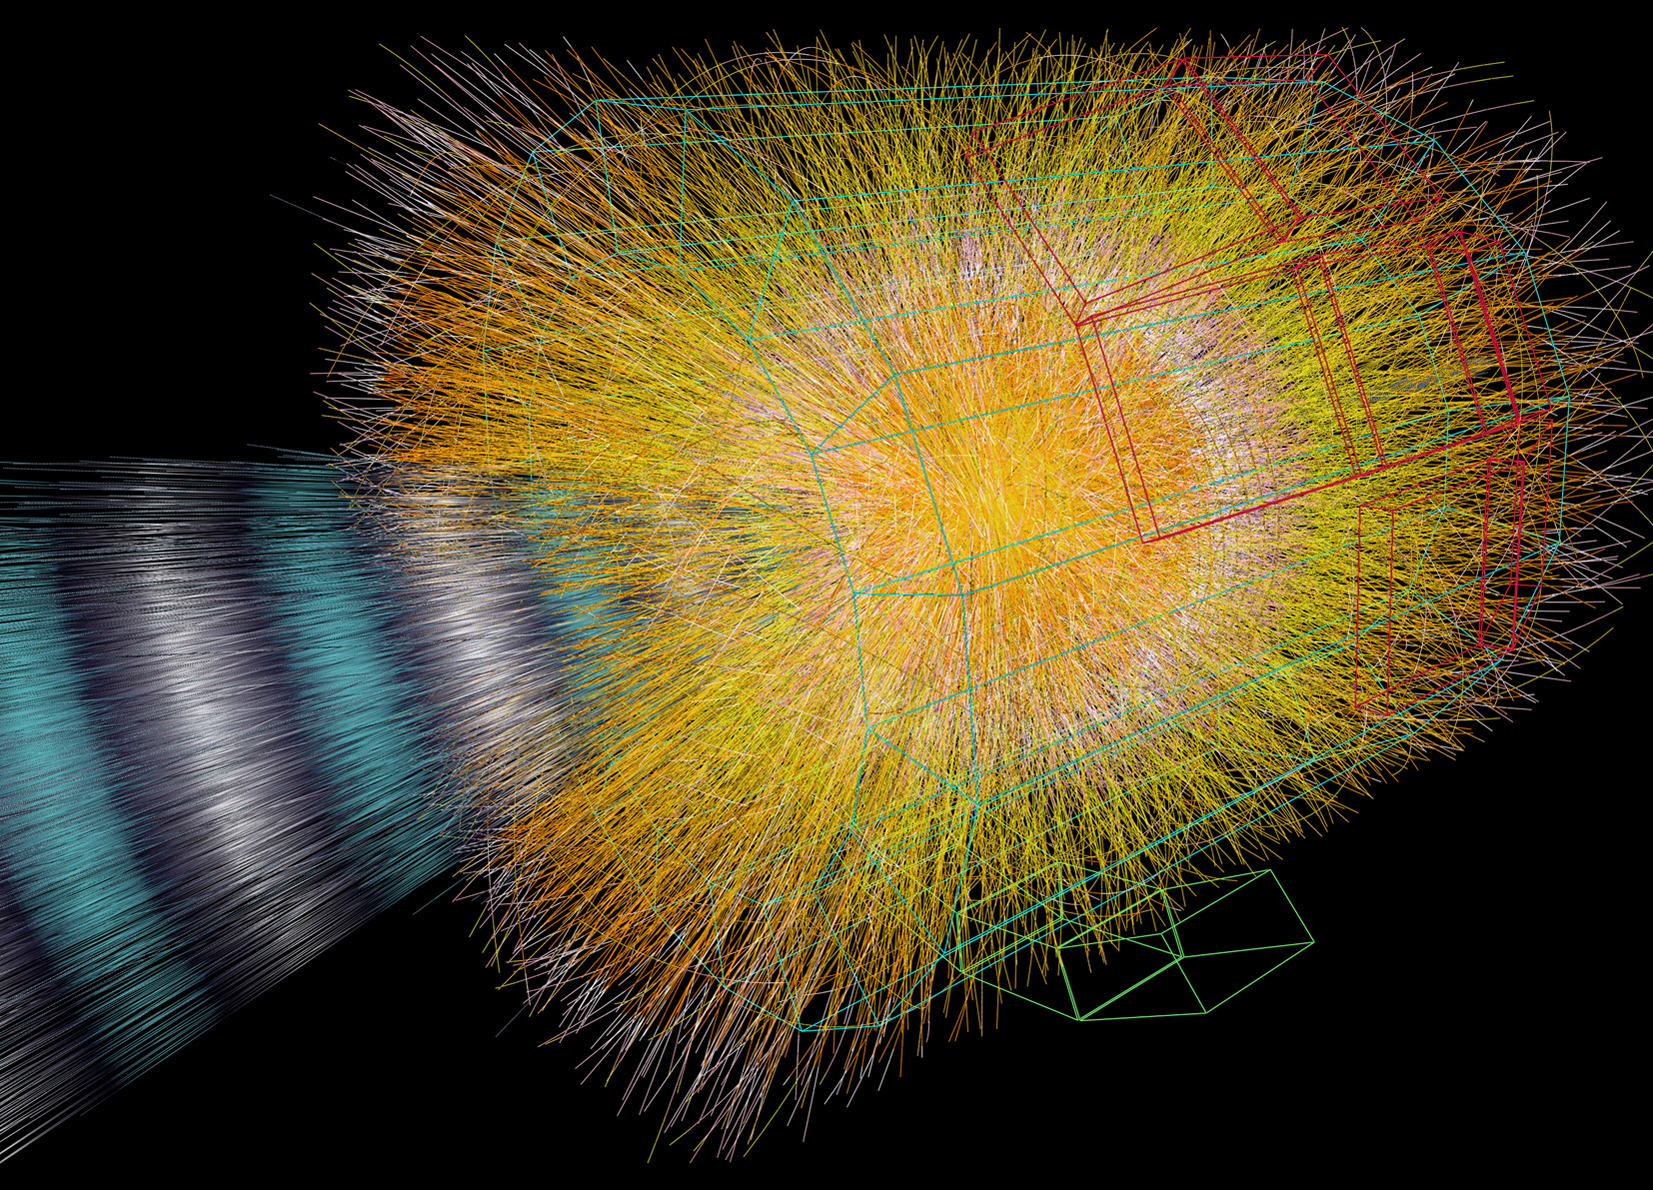
\includegraphics[width=\linewidth]{img/090324_ALICE-hirez.jpg}

\vspace{-11 cm}
\textcolor{white}{\hspace{0.25 cm} Combinatorics problem: tracks aren't labeled!}

\vspace{11 cm}
\end{columns}
\end{frame}

\begin{frame}{Finding a decay: ${K^0}_s \to \pi^+\pi^-$ example}
\large
\vspace{0.5 cm}
\begin{enumerate}
\item Loop over all pairs of particle tracks, tentatively labeling them $\pi^+$ and $\pi^-$.
\item Calculate $m = \sqrt{(E_{\pi^+} + E_{\pi^-})^2 - \left|\vec{p}_{\pi^+} + \vec{p}_{\pi^-}\right|^2}$ for each pair.
\end{enumerate}

\begin{center}
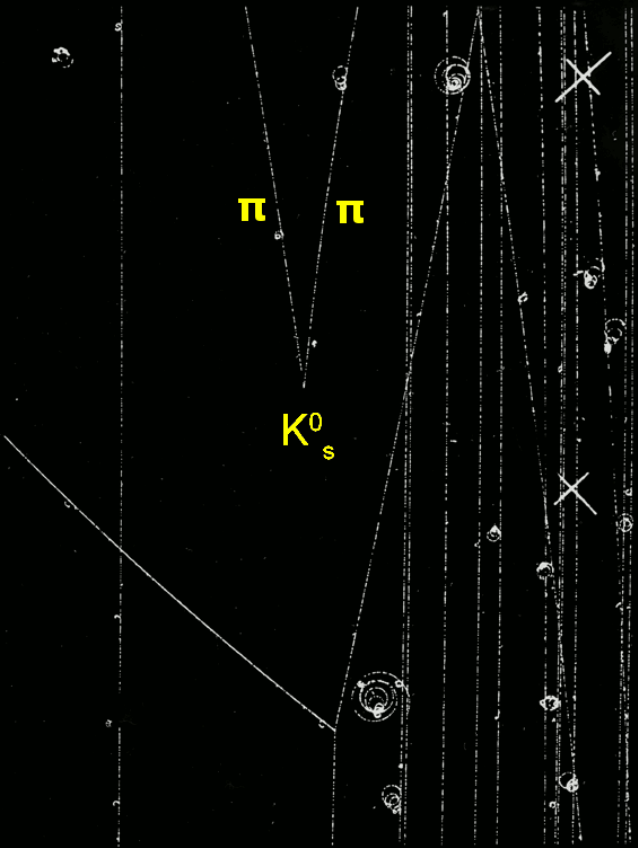
\includegraphics[height=4.2 cm]{img/kshort-1.png}\hspace{0.1 cm}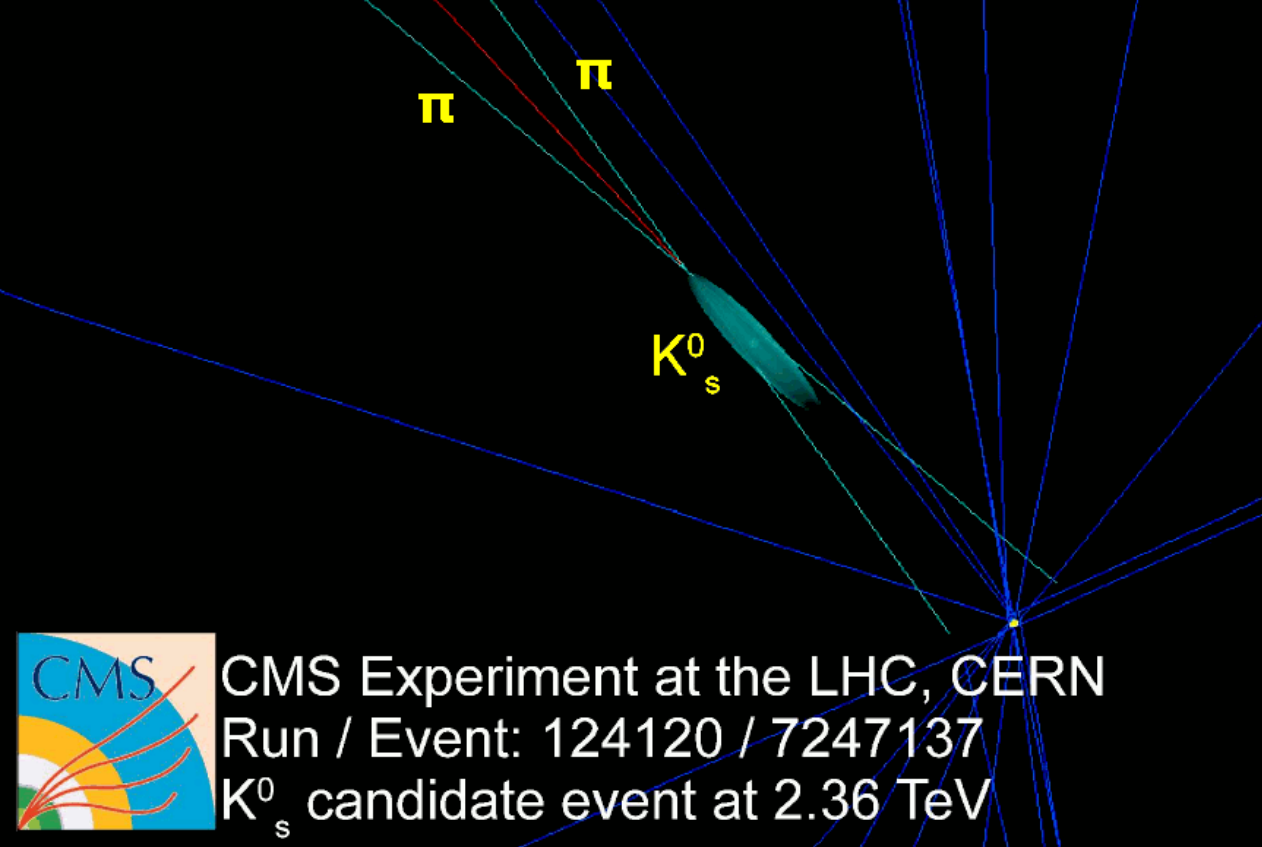
\includegraphics[height=4.2 cm]{img/kshort-2.png}\hspace{0.1 cm}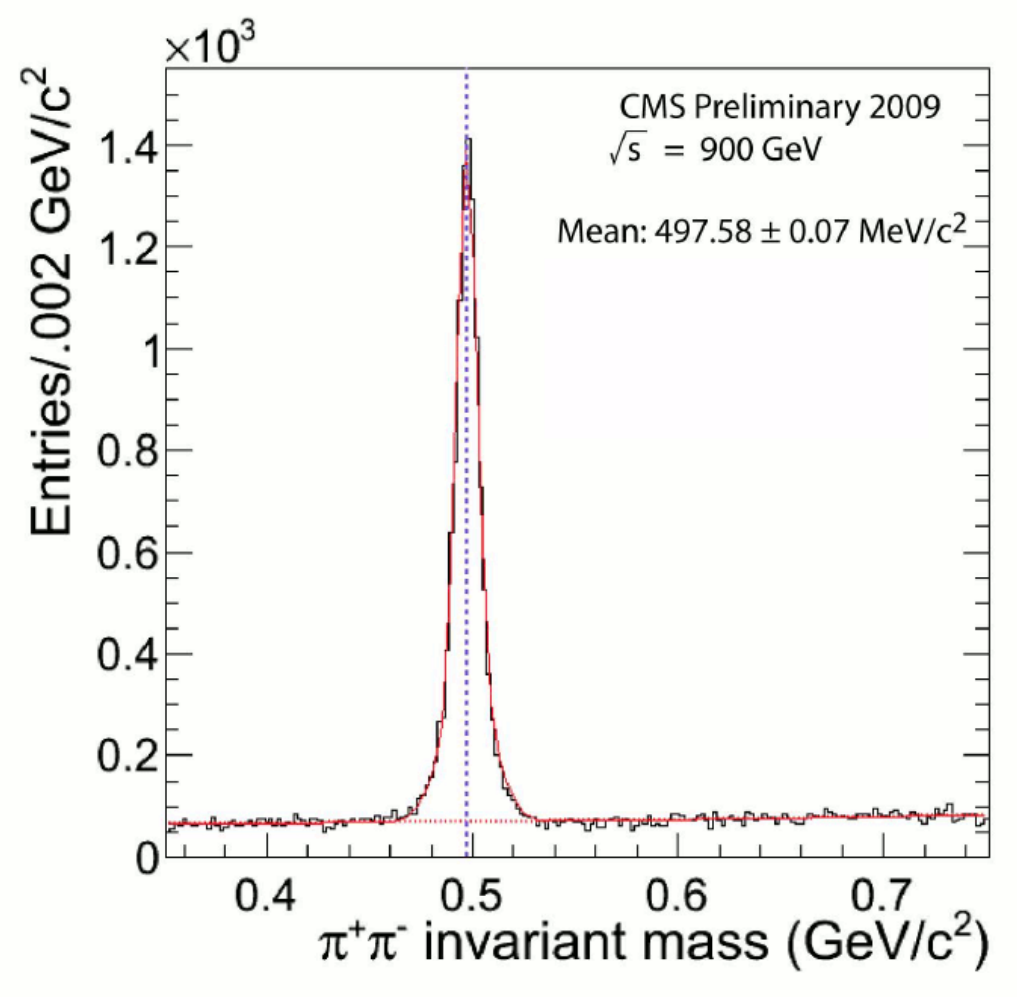
\includegraphics[height=4.2 cm]{img/kshort-3.png}
\end{center}

\begin{enumerate}\setcounter{enumi}{2}
\item The ones with $m \sim \mbox{mass}({{K^0}_s}) = 0.5\mbox{ GeV}/c^2$ are good candidates.
\end{enumerate}
\end{frame}

\begin{frame}{Apply the technique successively down the decay chain}
\Large
\begin{center}
$H \to ZZ$\hspace{1 cm}$Z \to e^+e^-$\hspace{1 cm}$Z \to \mu^+\mu^-$
\end{center}

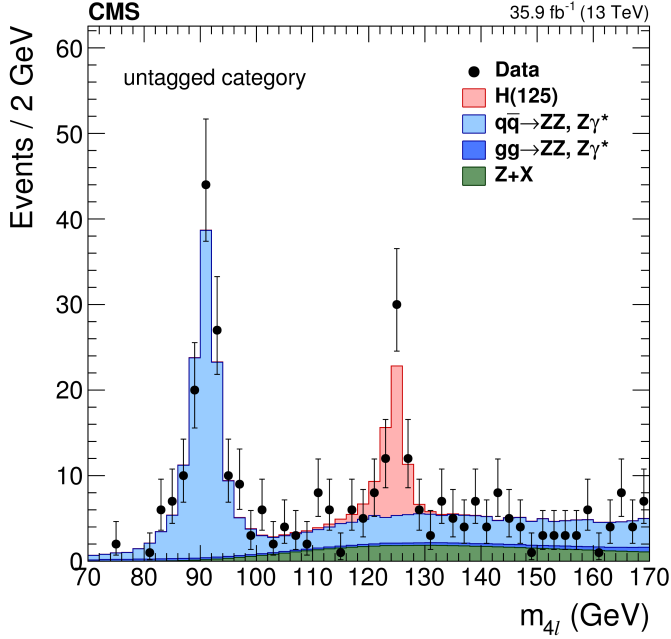
\includegraphics[height=6 cm]{img/higgs-to-four-leptons.png}\hfill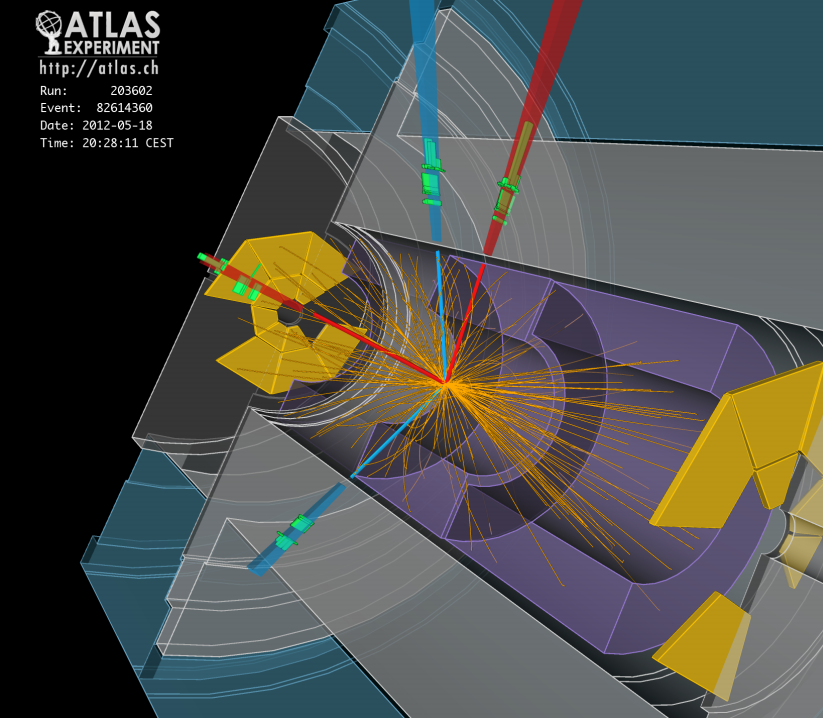
\includegraphics[height=6 cm]{img/higgs-to-four-leptons-2.png}
\end{frame}

\begin{frame}{Data structures are essential for this (and always have been)}
\large
\vspace{0.5 cm}

\vspace{0.25 cm}
\textcolor{darkblue}{{\it Initiation to Hydra} by R.K. B\"ock, 1976: added data structures to Fortran.}

\begin{center}
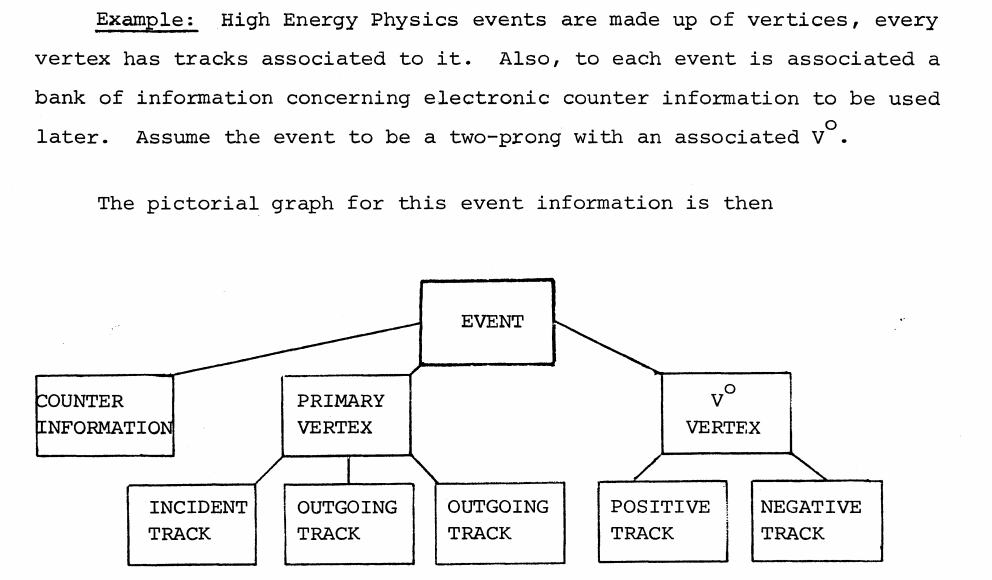
\includegraphics[width=0.7\linewidth]{img/hydra-3.png}
\end{center}
\end{frame}

\begin{frame}{Today, physicists use C++ and Python for analysis}
\large
\vspace{0.25 cm}

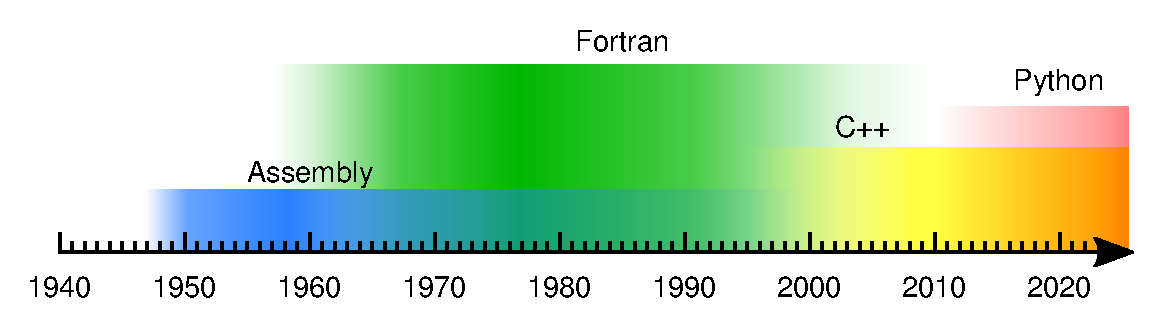
\includegraphics[width=\linewidth]{img/programming-languages.pdf}

\vspace{0.2 cm}
\begin{itemize}\setlength{\itemsep}{0.2 cm}
\item<2-> In C++, we can just write \mintinline{c++}{for} loops over data structures.
\item<3-> In Python, we have a difficult choice: NumPy is fast but limited to rectangular structures; pure Python is slow, but general.
\end{itemize}

\vspace{0.2 cm}
\Large
\begin{center}
\begin{minipage}{0.85\linewidth}
\begin{center}
\uncover<4->{Awkward Array provides NumPy-like interface and performance for general data structures.}
\end{center}
\end{minipage}
\end{center}
\end{frame}

\begin{frame}{}
\Huge
\vspace{1 cm}
\begin{center}
\textcolor{darkblue}{Exploring a dataset: Chicago bike paths}
\end{center}
\end{frame}

\begin{frame}{}
\Huge
\vspace{1 cm}
\begin{center}
\textcolor{darkblue}{Data types and extending NumPy}
\end{center}
\end{frame}

\begin{frame}{Data types \only<6->{and array features}}
\Large
\vspace{0.2 cm}

\begin{itemize}
\item<1-> \textcolor{darkblue}{Numerical:} what \mintinline{python}{np.ndarray} does: numbers, booleans, anything fixed-width.
\item<2-> \textcolor{darkblue}{Variable-length lists:} also known as ``jagged'' or ``ragged'' arrays.
\item<3-> \textcolor{darkblue}{Nested records:} with named (dict) or unnamed (tuple) fields.
\item<4-> \textcolor{darkblue}{Option type:} nullable/masked data; values that can be \mintinline{python}{None}.
\item<5-> \textcolor{darkblue}{Union type:} heterogeneous data; different types in one array.
\end{itemize}

\vspace{0.25 cm}
\begin{itemize}
\item<6-> \textcolor{darkblue}{Indirection:} can be used to enumerate categorical values.
\item<7-> \textcolor{darkblue}{Partitioning:} chunks of an array can be processed in parallel.
\item<8-> \textcolor{darkblue}{Virtualness:} they can also be lazily loaded.
\item<9-> \textcolor{darkblue}{Behaviors:} arrays and records with domain-specific meaning, like ``spacetime point'' or ``string'' can be given specialized methods.
\end{itemize}
\end{frame}

\begin{frame}[fragile]{Generalizing NumPy: broadcasting}
\begin{center}
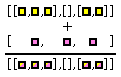
\includegraphics[width=0.4\linewidth]{img/cartoon-broadcasting.pdf}
\end{center}

\begin{columns}
\column{1.03\linewidth}
\begin{minted}{python}
>>> jagged = ak.Array([[1, 2, 3],  [], [4, 5]])
>>> flat   = ak.Array([      100, 200,    300])
>>> jagged + flat
<Array [[101, 102, 103], [], [304, 305]] type='3 * var * int64'>
\end{minted}
\end{columns}
\end{frame}

\begin{frame}[fragile]{Generalizing NumPy: reduction}
\vspace{0.5 cm}

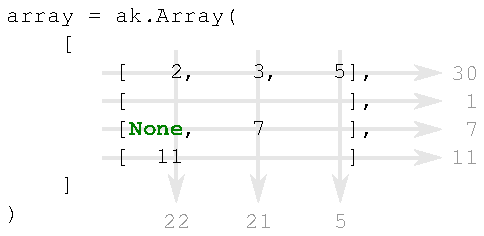
\includegraphics[width=8 cm]{img/reduction.pdf}

%% \begin{minted}{python}
%% array = ak.Array(
%%     [
%%         [   2,    3,    5],
%%         [                ],
%%         [None,    7      ],
%%         [  11            ]
%%     ]
%% )
%% \end{minted}

\begin{minted}{python}
>>> ak.prod(array, axis=0)
<Array [22, 21, 5] type='3 * int64'>
\end{minted}

\begin{minted}{python}
>>> ak.prod(array, axis=1)
<Array [30, 1, 7, 11] type='4 * int64'>
\end{minted}
\end{frame}

\begin{frame}[fragile]{Generalizing NumPy: slices}
\vspace{0.25 cm}

\begin{minted}{python}
array = ak.Array([
    [{"x": 1,  "y": [101]},
     {"x": 4,  "y": [102, 202]},
     {"x": 9,  "y": [103, 203, 303]}],
    [],
    [{"x": 16, "y": [104, 204, 304, 404]},
     {"x": 25, "y": [105, 205, 305, 405, 505]}]
])
\end{minted}

\begin{onlyenv}<1>
\vspace{0.25 cm}
\begin{minted}{python}
>>> array[2, 1, "y", 0]
105
>>> array[2, "y", 1, 0]
105
>>> array["y", 2, 1, 0]
105
\end{minted}
\vspace{5 cm}
\end{onlyenv}

\begin{onlyenv}<2>
\vspace{0.25 cm}
\begin{minted}{python}
>>> array["x"]
<Array [[1, 4, 9], [], [16, 25]] type='3 * var * int64'>
\end{minted}
\vspace{5 cm}
\end{onlyenv}

\begin{onlyenv}<3>
\vspace{0.25 cm}
\begin{minted}{python}
>>> array.x % 2 == 0
<Array [[False, True, False], [], [True, False]] type='3 * var * bool'>
\end{minted}

\vspace{0.25 cm}
\begin{minted}{python}
>>> array.x[array.x % 2 == 0]
<Array [[4], [], [16]] type='3 * var * int64'>
\end{minted}
\vspace{5 cm}
\end{onlyenv}
\end{frame}

\begin{frame}[fragile]{Generalizing NumPy: completely new functions}
\scriptsize
\vspace{0.5 cm}

\begin{columns}
\column{0.5\linewidth}
\textcolor{darkblue}{\Large Cartesian product}

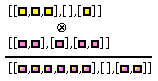
\includegraphics[width=\linewidth]{img/cartoon-cartesian.pdf}

\begin{minted}{python}
>>> x = [[1, 2, 3], [], [4]]
>>> y = [["a", "b"], ["c"], ["d", "e"]]
>>> ak.cartesian([x, y], axis=1)
[[(1, "a"), (1, "b"),
  (2, "a"), (2, "b"),
  (3, "a"), (3, "b")],
 [],
 [(4, "d"), (4, "e")]]
\end{minted}

\column{0.52\linewidth}
\textcolor{darkblue}{\Large Combinations without replacement}

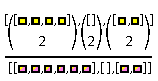
\includegraphics[width=\linewidth]{img/cartoon-combinations.pdf}

\begin{minted}{python}
>>> x = [[1, 2, 3, 4], [], [5, 6]]
>>> ak.combinations(x, 2, axis=1)
[[(1, 2), (1, 3), (1, 4),
  (2, 3), (2, 4), (3, 4)],
 [],
 [(5, 6)]]
\end{minted}
\vspace{\baselineskip}
\end{columns}
\end{frame}

\begin{frame}{}
\Huge
\vspace{1 cm}
\begin{center}
\textcolor{darkblue}{Using Awkward Arrays in Numba}
\end{center}
\end{frame}

\begin{frame}[fragile]{Awkward Arrays can be used in Numba-compiled functions}
\vspace{0.1 cm}
\small
\begin{minted}{python}
import numba as nb                  #  50× faster than ak.sum version
@nb.jit                             # 250× faster than the pure Python
def compute_lengths(bikeroutes):
    route_length = np.zeros(len(bikeroutes.features))
    for i in range(len(bikeroutes.features)):
        for path in bikeroutes.features[i].geometry.coordinates:
            first = True
            last_east, last_north = 0.0, 0.0
            for lng_lat in path:
                km_east = lng_lat[0] * 82.7
                km_north = lng_lat[1] * 111.1
                if not first:
                    dx2 = (km_east - last_east)**2
                    dy2 = (km_north - last_north)**2
                    route_length[i] += np.sqrt(dx2 + dy2)
                first = False
                last_east, last_north = km_east, km_north
    return route_length
\end{minted}
\end{frame}

\begin{frame}{\mbox{ }}
\vspace{0.5 cm}
\large
\begin{columns}
\column{0.0125\linewidth}

\column{0.55\linewidth}
\textcolor{darkblue}{\Large Awkward Array by itself}

\vspace{0.25 cm}
\begin{itemize}\setlength{\itemsep}{0.2 cm}
\item<1-> Array-based programming
\item<2-> Some calculations are more succinct, easier to read as expressions
\item<3-> Precompiled operations
\item<4-> Complex formul\ae\ require intermediate arrays, multiple passes over data
\item<5-> Easy to generate complex output \mbox{\hspace{2 cm}}
\end{itemize}

\column{0.55\linewidth}
\textcolor{darkblue}{\Large Awkward Array with Numba}

\vspace{0.25 cm}
\begin{itemize}\setlength{\itemsep}{0.2 cm}
\item<1-> Imperative (Python) programming
\item<2-> Others are easier to read as algorithms, especially ``iterate until converged''
\item<3-> Just-in-time compiled (one-time cost)
\item<4-> Number of passes over the data depends on \mintinline{python}{for} loops
\item<5-> Complex output requires a new mechanism
\end{itemize}
\end{columns}
\end{frame}

\begin{frame}[fragile]{ArrayBuilder (can be used in Numba)}
\vspace{0.1 cm}
\scriptsize
\begin{columns}
\column{1.1\linewidth}
\begin{uncoverenv}<1->
\begin{minted}{python}
b = ak.ArrayBuilder()
\end{minted}
\end{uncoverenv}
\vspace{-0.25 cm}
\begin{uncoverenv}<2->
\begin{minted}{python}
b.begin_list()    # [         # 0 * var * unknown     (initially, the type is unknown)
\end{minted}
\end{uncoverenv}
\vspace{-0.43 cm}
\begin{uncoverenv}<3->
\begin{minted}{python}
b.integer(1)      #   1,      # 0 * var * int64
\end{minted}
\end{uncoverenv}
\vspace{-0.43 cm}
\begin{uncoverenv}<4->
\begin{minted}{python}
b.integer(2)      #   2,      # 0 * var * int64
\end{minted}
\end{uncoverenv}
\vspace{-0.43 cm}
\begin{uncoverenv}<5->
\begin{minted}{python}
b.real(3)         #   3.0     # 0 * var * float64     (all the integers have become floats)
\end{minted}
\end{uncoverenv}
\vspace{-0.43 cm}
\begin{uncoverenv}<6->
\begin{minted}{python}
b.end_list()      # ],        # 1 * var * float64
\end{minted}
\end{uncoverenv}
\vspace{-0.43 cm}
\begin{uncoverenv}<7->
\begin{minted}{python}
b.begin_list()    # [         # 1 * var * float64
\end{minted}
\end{uncoverenv}
\vspace{-0.43 cm}
\begin{uncoverenv}<8->
\begin{minted}{python}
b.end_list()      # ],        # 2 * var * float64
\end{minted}
\end{uncoverenv}
\vspace{-0.43 cm}
\begin{uncoverenv}<9->
\begin{minted}{python}
b.begin_list()    # [         # 2 * var * float64
\end{minted}
\end{uncoverenv}
\vspace{-0.43 cm}
\begin{uncoverenv}<10->
\begin{minted}{python}
b.integer(4)      #   4,      # 2 * var * float64
\end{minted}
\end{uncoverenv}
\vspace{-0.43 cm}
\begin{uncoverenv}<11->
\begin{minted}{python}
b.null()          #   null    # 2 * var * ?float64    (now the floats are nullable)
\end{minted}
\end{uncoverenv}
\vspace{-0.43 cm}
\begin{uncoverenv}<12->
\begin{minted}{python}
b.end_list()      # ],        # 3 * var * ?float64
\end{minted}
\end{uncoverenv}
\vspace{-0.43 cm}
\begin{uncoverenv}<13->
\begin{minted}{python}
b.begin_list()    # [         # 3 * var * ?float64
\end{minted}
\end{uncoverenv}
\vspace{-0.43 cm}
\begin{uncoverenv}<14->
\begin{minted}{python}
b.begin_record()  #   {       # 3 * var * ?union[float64, {}]
\end{minted}
\end{uncoverenv}
\vspace{-0.43 cm}
\begin{uncoverenv}<15->
\begin{minted}{python}
b.field("x")      #     "x":  # 3 * var * ?union[float64, {"x": unknown}]
\end{minted}
\end{uncoverenv}
\vspace{-0.43 cm}
\begin{uncoverenv}<16->
\begin{minted}{python}
b.integer(1)      #      1,   # 3 * var * ?union[float64, {"x": int64}]
\end{minted}
\end{uncoverenv}
\vspace{-0.43 cm}
\begin{uncoverenv}<17->
\begin{minted}{python}
b.field("y")      #      "y": # 3 * var * ?union[float64, {"x": int64, "y": unknown}]
\end{minted}
\end{uncoverenv}
\vspace{-0.43 cm}
\begin{uncoverenv}<18->
\begin{minted}{python}
b.begin_list()    #      [    # 3 * var * ?union[float64, {"x": int64, "y": var * unknown}]
\end{minted}
\end{uncoverenv}
\vspace{-0.43 cm}
\begin{uncoverenv}<19->
\begin{minted}{python}
b.integer(2)      #        2, # 3 * var * ?union[float64, {"x": int64, "y": var * int64}]
\end{minted}
\end{uncoverenv}
\vspace{-0.43 cm}
\begin{uncoverenv}<20->
\begin{minted}{python}
b.integer(3)      #        3  # 3 * var * ?union[float64, {"x": int64, "y": var * int64}]
\end{minted}
\end{uncoverenv}
\vspace{-0.43 cm}
\begin{uncoverenv}<21->
\begin{minted}{python}
b.end_list()      #      ]    # 3 * var * ?union[float64, {"x": int64, "y": var * int64}]
\end{minted}
\end{uncoverenv}
\vspace{-0.43 cm}
\begin{uncoverenv}<22->
\begin{minted}{python}
b.end_record()    #   }       # 3 * var * ?union[float64, {"x": int64, "y": var * int64}]
\end{minted}
\end{uncoverenv}
\vspace{-0.43 cm}
\begin{uncoverenv}<23->
\begin{minted}{python}
b.end_list()      # ]         # 4 * var * ?union[float64, {"x": int64, "y": var * int64}]
\end{minted}
\end{uncoverenv}
\end{columns}
\end{frame}

\begin{frame}{}
\Huge
\vspace{1 cm}
\begin{center}
\textcolor{darkblue}{How it works: columnar transformations}
\end{center}
\end{frame}

\begin{frame}[fragile]{Columnar data structures}
\vspace{0.5 cm}

\begin{onlyenv}<1-3>
\begin{Verbatim}[commandchars=\\\{\}]
array = ak.Array([
    \textcolor{red}{[}\{\textcolor{darkgray}{"x"}: \textcolor{darkgreen}{1},  \textcolor{darkgray}{"y"}: \textcolor{blue}{[}\textcolor{darkorange}{11}\textcolor{blue}{]}\},
     \{\textcolor{darkgray}{"x"}: \textcolor{darkgreen}{4},  \textcolor{darkgray}{"y"}: \textcolor{blue}{[}\textcolor{darkorange}{12, 22}\textcolor{blue}{]}\},
     \{\textcolor{darkgray}{"x"}: \textcolor{darkgreen}{9},  \textcolor{darkgray}{"y"}: \textcolor{blue}{[}\textcolor{darkorange}{13, 23, 33}\textcolor{blue}{]}\}\textcolor{red}{]},
    \textcolor{red}{[]},
    \textcolor{red}{[}\{\textcolor{darkgray}{"x"}: \textcolor{darkgreen}{16}, \textcolor{darkgray}{"y"}: \textcolor{blue}{[}\textcolor{darkorange}{14, 24, 34, 44}\textcolor{blue}{]}\}\textcolor{red}{]}
])
\end{Verbatim}
\end{onlyenv}\begin{onlyenv}<4>
\begin{Verbatim}[commandchars=\\\{\}]
array = ak.Array([
    \textcolor{red}{[}\{\textcolor{darkgray}{"x"}: \textcolor{darkgreen}{1},  \textcolor{darkgray}{"y"}: \textcolor{blue}{[}\textcolor{darkorange}{  }\textcolor{blue}{]}\},
     \{\textcolor{darkgray}{"x"}: \textcolor{darkgreen}{4},  \textcolor{darkgray}{"y"}: \textcolor{blue}{[}\textcolor{darkorange}{    22}\textcolor{blue}{]}\},
     \{\textcolor{darkgray}{"x"}: \textcolor{darkgreen}{9},  \textcolor{darkgray}{"y"}: \textcolor{blue}{[}\textcolor{darkorange}{    23, 33}\textcolor{blue}{]}\}\textcolor{red}{]},
    \textcolor{red}{[]},
    \textcolor{red}{[}\{\textcolor{darkgray}{"x"}: \textcolor{darkgreen}{16}, \textcolor{darkgray}{"y"}: \textcolor{blue}{[}\textcolor{darkorange}{    24, 34, 44}\textcolor{blue}{]}\}\textcolor{red}{]}
])
\end{Verbatim}
\end{onlyenv}

\begin{onlyenv}<1>
\vspace{0.25 cm}
\begin{Verbatim}[commandchars=\\\{\}]
outer offsets:  \textcolor{red}{0,                     3,  3, 5}
content for x:  \textcolor{darkgreen}{1,  4,      9,            16}
offsets for y:  \textcolor{blue}{0,  1,      3,             6,            10}
content for y: \textcolor{darkorange}{11, 12, 22, 13, 23, 33,    14, 24, 34, 44}
\end{Verbatim}
\vspace{5 cm}
\end{onlyenv}\begin{onlyenv}<2>
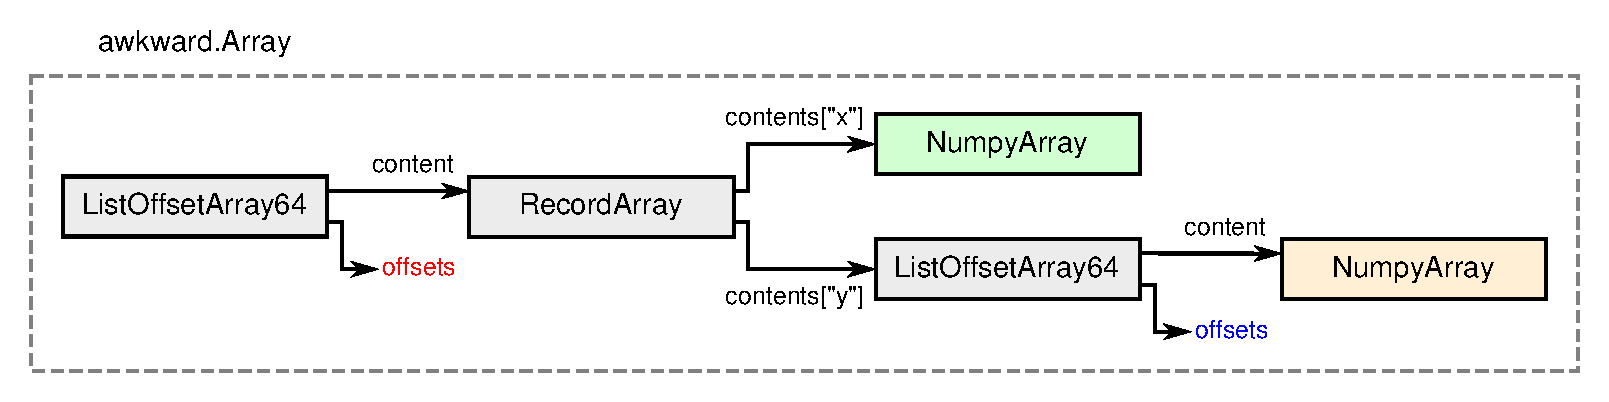
\includegraphics[width=\linewidth]{img/example-hierarchy.pdf}
\vspace{5 cm}
\end{onlyenv}\begin{onlyenv}<3>
\vspace{0.25 cm}
\begin{minted}{python}
>>> array[:, :, "y", 1:]
\end{minted}

\vspace{0.25 cm}
\begin{Verbatim}[commandchars=\\\{\}]
outer offsets:  \textcolor{red}{0,                     3,  3, 5}
content for x:  \textcolor{darkgreen}{1,  4,      9,            16}
starts  for y:  \textcolor{blue}{0,  1,      3,             6}
stops   for y:  \textcolor{blue}{    1,      3,             6,            10}
content for y: \textcolor{darkorange}{11, 12, 22, 13, 23, 33,    14, 24, 34, 44}
\end{Verbatim}
\vspace{5 cm}
\end{onlyenv}\begin{onlyenv}<4>
\vspace{0.25 cm}
\begin{minted}{python}
>>> array[:, :, "y", 1:]
\end{minted}

\vspace{0.25 cm}
\begin{Verbatim}[commandchars=\\\{\}]
outer offsets:  \textcolor{red}{0,                     3,  3, 5}
content for x:  \textcolor{darkgreen}{1,  4,      9,            16}
starts  for y:  \textcolor{blue}{    1,  2,      4,             7}
stops   for y:  \textcolor{blue}{    1,      3,             6,            10}
content for y: \textcolor{darkorange}{11, 12, 22, 13, 23, 33,    14, 24, 34, 44}
\end{Verbatim}
\vspace{5 cm}
\end{onlyenv}

\end{frame}



%% \begin{frame}{Like Apache Arrow, but for data transformations}
%% \vspace{0.25 cm}
%% \begin{columns}
%% \column{1.1\linewidth}
%% 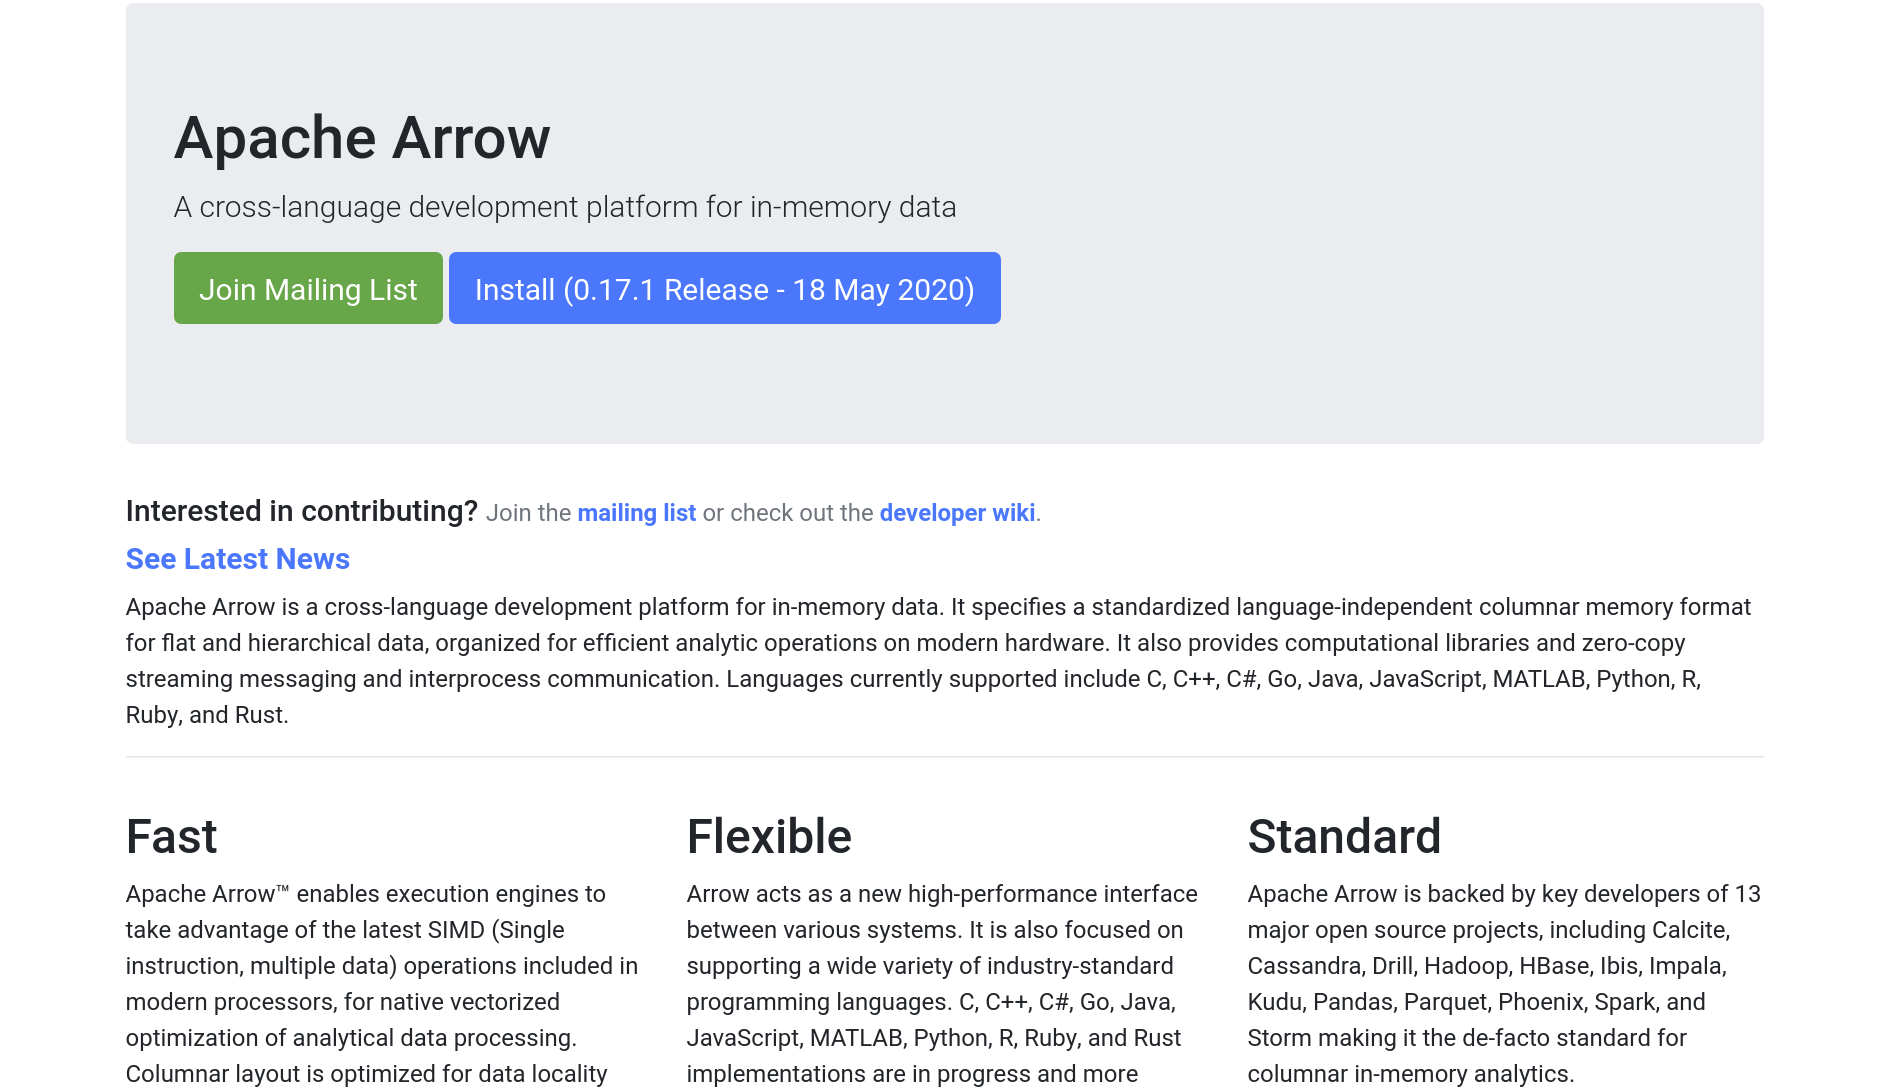
\includegraphics[width=\linewidth]{img/apache-arrow.png}
%% \end{columns}
%% \end{frame}

\end{document}
